\section{Benchmark Suite}

%% Over the past eight years, we have gained considerable experience in
%% developing applications in StreamIt.  We reflect on this experience
%% first via a quantitative analysis of our benchmark suite, and then via
%% qualitative impressions from StreamIt programmers.

An overview of the StreamIt benchmark suite appears in
Table~\ref{tab:lang-benchmarks}.  At the time of this writing, the
suite consists of 67 programs, including 29 realistic applications, 4
graphics rendering pipelines, 19 libraries and kernels, 8 sorting
routines, and 7 toy examples.  Benchmarks range in size from 21 lines
(Fibonacci) to over 4,000 lines (MPEG2 encoder), with a total of
33,800 non-comment, non-blank lines in the suite\footnotemark[1].
Over 20 people contributed to the suite, including 6 from outside our
group.
%% median-pulse compression doppler radar was developed at Halmstad
%% University~\cite{ola-techrep}, TDE was developed at the Information
%% Sciences Insittute, an FFT and bitonic sort were developed at UC
%% Berkeley~\cite{mani-permutations}, and the graphics pipelines were
%% implemented primarily by the graphics group at
%% MIT~\cite{chen-graphics05}.  
%%
%% OFDM was adapted from an internal performance test of
%% Spectrumware~\cite{tennenhouse_spectrumware_1996}, while Vocoder was
%% implemented with support from Seneff~\cite{seneff80thesis}.  Other 
Benchmarks were often adapted from a reference implementation in C,
Java, or MATLAB.

Graphical depictions of the stream graphs for each benchmark can be
found in an accompanying report~\cite{thies-thesis}.
%the complete source
%code for a small benchmark (ChannelVocoder) can be found in
%Appendix~\ref{chap:example-program}.  
A subset of the benchmarks have also been prepared for public release
on the StreamIt website~\cite{streamitweb}.  At the time of this
writing, some of the larger benchmarks (MPEG2, GMTI, Mosaic, FAT,
HDTV) are not fully supported by the compiler.  However, their
functional correctness has been verified in the Java runtime for the
StreamIt language.

It is important to recognize that most of the benchmarks are
parameterized, and we study only one assignment of those parameters in
our quantitative evaluation.  Table~\ref{tab:lang-benchmarks} details
the parameterization of the StreamIt benchmarks.  In two-thirds (44)
of the benchmarks, the parameters affect the structure of the stream
graph, often by influencing the length of pipelines, the width of
splitjoins, the depth of recursion hierarchies, or the absence or
presence of given filters.  The same number of benchmarks contain
parameters that affect the I/O rates of filters (e.g., the length of
an FIR filter), but do not necessarily affect the structure of the
graph.  Changes to the I/O rates also imply changes to the schedule
and possibly the balance of work across filters.  In selecting values
for these parameters, our primary goal was to faithfully represent a
real-life application of the algorithm.  In some cases we also
decreased the sizes of the parameters (e.g., sorting 16 elements at a
time) to improve the comprehensibility of the stream graph.  For
benchmarking purposes, researchers may wish to scale up the parameters
to yield larger graphs, or to vary the ratio between parameters to
obtain graphs of varying shapes and work distributions.

More detailed properties of the filters and streams within each
benchmark are given in Table~\ref{tab:lang-benchmarks-filters}.  In
terms of size, benchmarks declare (on average) 11 filter types and
instantiate them 63 times in the stream graph.  GMTI contains the most
filters, with 95 static types and 1,111 dynamic instances; it also
contains 1,757 instances of the Identity filter, to assist with data
reordering.

\footnotetext[1]{Counting commented lines (8,000) and blank lines
  (7,300), the benchmark suite comes to 49,300 lines.}

\begin{table*}[t!]
\hspace{-0.3in}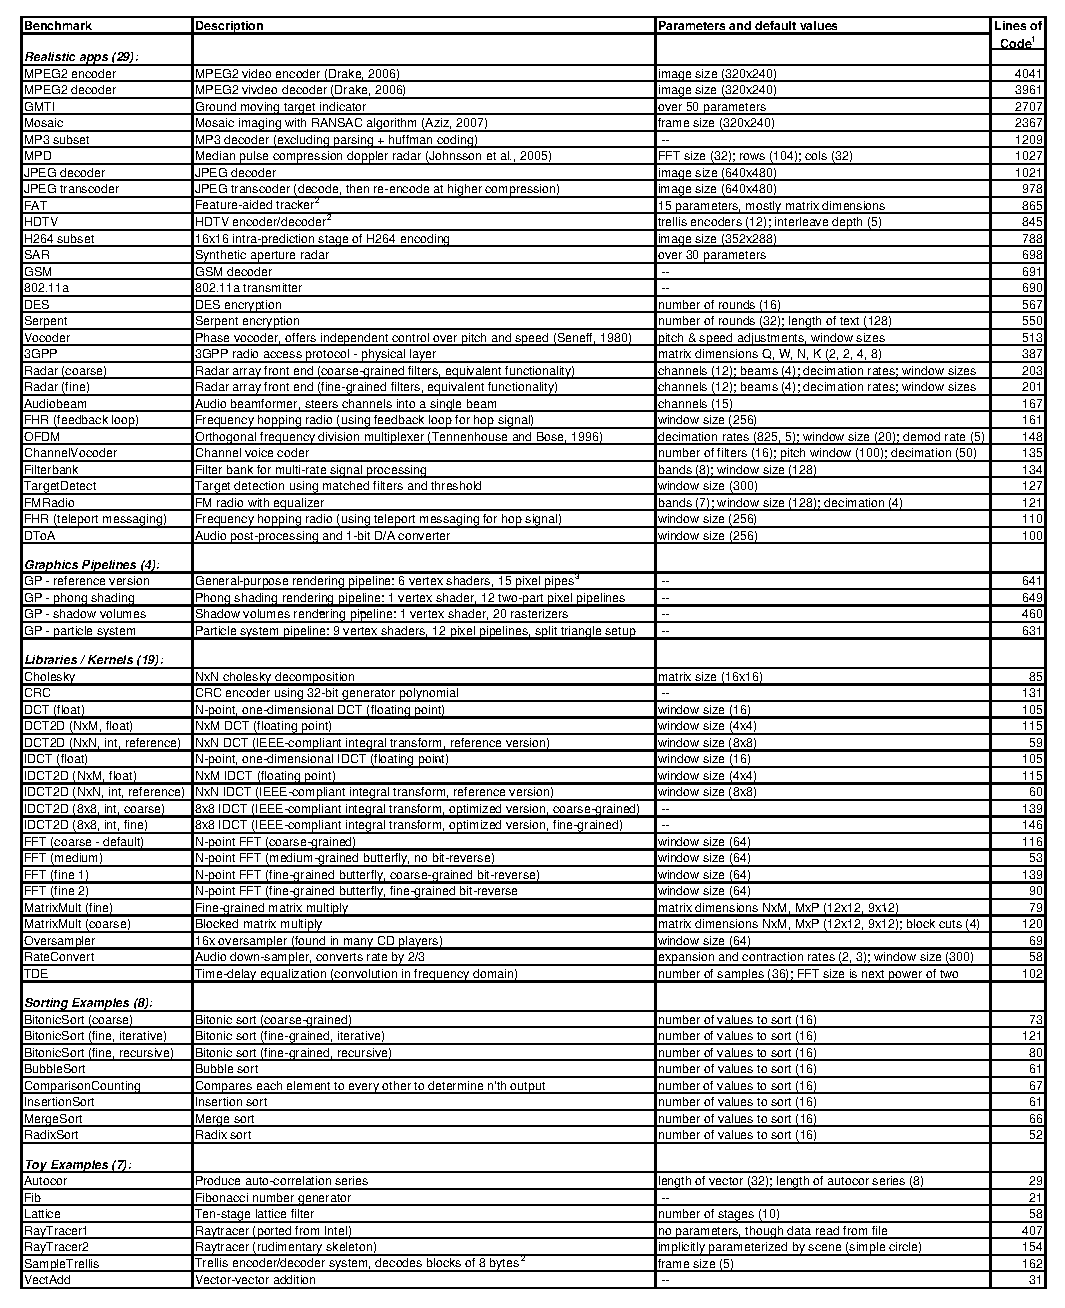
\psfig{file=benchmarks,height=\textheight}
\vspace{-12pt}
\caption{Overview of the StreamIt benchmark suite.\protect\label{tab:lang-benchmarks}}
\vspace{-0.5in}
\end{table*}

\begin{table*}[t!]
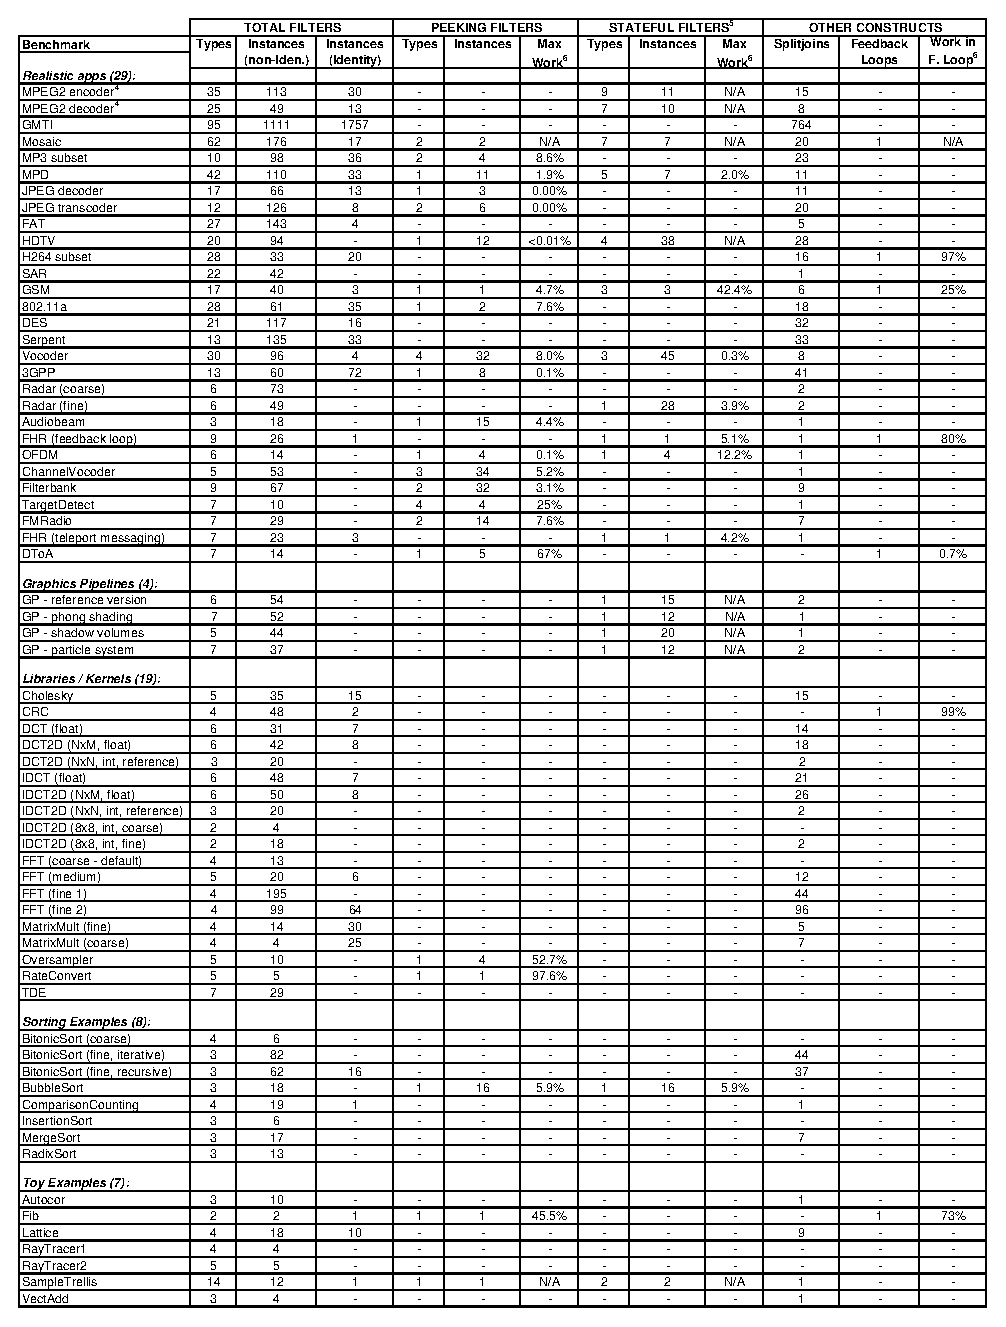
\psfig{file=benchmarks-filters,width=\textwidth}
\vspace{-12pt}
\caption{Properties of filters and other constructs in StreamIt 
benchmarks.\protect\label{tab:lang-benchmarks-filters}}
\vspace{-0.5in}
\end{table*}
